%28/01 - Aythami Morales 
\chapter{Introducción}
\section{Repaso: Álgebra lineal}
\subsection{Notación general}
Se denota un \textbf{vector} $\vec{x}$ como $x \in \mathbb{R}^n$ con $n$ entradas, donde $x_i \in \mathbb{R}$ es la entrada i-ésima. Un vector se puede ver como una matriz de dimensiones $n \times 1$ y se denomina también como vector-columna.
$$\vec{x} = \begin{pmatrix}
x_1 \\ x_2 \\ ... \\ x_n
\end{pmatrix} \in \mathbb{R}^n$$

Se denota una \textbf{matriz} $\vec{A}$ como $A \in \mathbb{R}^{m \times n}$ con n columnas y m filas, donde $A_{i,j} \in \mathbb{R}$ es la entrada en la fila i-ésima y columna j-ésima.
$$\vec{A} = \begin{pmatrix}
A_{1,1} & ... & A_{1,n} \\
... & & ...\\
A_{m,1} & ... & A_{m,n}
\end{pmatrix} \in \mathbb{R}^{m \times n}$$

Una \textbf{matriz de identidad} $\vec{I} \in \mathbb{R}^{n \times n}$ es una matriz cuadrada con 1 en la diagonal principal y 0 en el resto. Para cualquier matriz $\vec{A} \in \mathbb{R}^{n \times n}$, se cumple que $\vec{A} \times \vec{I} = \vec{I} \times \vec{A} = \vec{A}$.
$$\vec{I} = \begin{pmatrix}
1 & 0 & ... & 0 \\
0 & 1 & ... & ... \\
... & ... & 1 & 0 \\
0 & ... & 0 & 1
\end{pmatrix}$$

\subsection{Operaciones de matrices}
\paragraph{Multiplicación vector-vector}
Hay dos tipos de productos vector-vector:
\begin{itemize}
\item \textbf{Producto interno (inner product):}
Dados dos vectores $\vec{x},\vec{y} \in \mathbb{R}^n$ de la misma dimensión, el producto interno es un escalar (un sólo número). Se usa en cálculos que involucran proyecciones, determinación de ortogonalidad, etc. El producto interno puede aplicarse en cualquier dimensión.
$$\vec{x}^T y = \sum^n_{i=1} x_iy_i \in \mathbb{R} $$

\item \textbf{Producto externo (outer product):}
Dados dos vectores, no necesariamente de la misma dimensión, $\vec{x} \in \mathbb{R}^m, \vec{y} \in \mathbb{R}^n$, el producto externo es una matriz de $m \times n$.
$$xy^T = \begin{pmatrix}
x_1 y_1 & ... & x_1 y_n \\
...  & & ... \\
x_m y_1 & ... & x_m y_n
\end{pmatrix} \in \mathbb{R}^{m \times n}$$

El producto externo tiene las siguientes aplicaciones en bioinformática:
\begin{itemize}
\item \textbf{Álgebra lineal}
\begin{itemize}
\item \textbf{Matrices de Covarianza}: Se utiliza en la construcción de matrices de covarianza, que son fundamentales en estadística y análisis de datos.
\item \textbf{Representación de Transformaciones}: Ayuda a representar transformaciones lineales y rotaciones en el espacio.
\end{itemize}
\item \textbf{Análisis de Datos y Machine Learning}
\begin{itemize}
\item \textbf{Modelos de Regresión}: En algunos métodos de regresión, como la regresión de mínimos cuadrados, se utiliza el producto externo para construir matrices de diseño.
\item \textbf{Métodos de Factorización}: Se aplica en técnicas como la factorización de matrices y la descomposición en valores singulares (SVD), que son esenciales en la reducción de dimensionalidad y análisis de componentes principales (PCA).
\end{itemize}
\end{itemize}
\end{itemize}

\paragraph{Multiplicación matriz-vector} Dada una matriz $\vec{A} \in \mathbb{R}^{m \times n}$ y un vector $\vec{x} \in \mathbb{R}^n$, el producto es un vector del tamaño $\mathbb{R}^m$. El proceso consiste en multiplicar cada fila de la matriz $\vec{A}$ por el vector $\vec{x}$ y sumar los resultados.
$$Ax = \begin{pmatrix}
A_{1,1}x_1 + A_{1,2}x_2 + ... + A_{1,n}x_n \\
... \\
A_{m,1}x_1 + A_{m,2}x_2 + ... + A_{m,n}x_n
\end{pmatrix} \in \mathbb{R}^m$$

\begin{figure}[h]
\centering
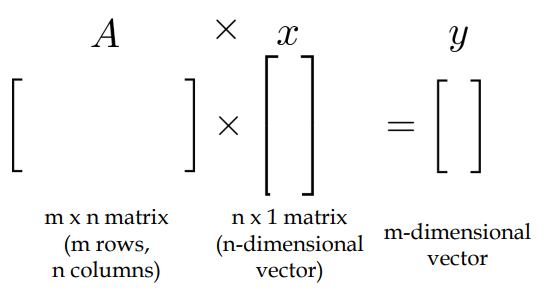
\includegraphics[width = 0.5\textwidth]{figs/matrix-vector-mult.png}
\end{figure}

Entre las aplicaciones de la multiplicación matriz-vector se encuentran:
\begin{itemize}
\item \textbf{Álgebra lineal y matemáticas puras}
\begin{itemize}
\item \textbf{Sistemas de Ecuaciones Lineales}: Resolver sistemas de ecuaciones de la forma \(Ax = b\).
\item \textbf{Transformaciones Lineales}: Representar y aplicar transformaciones lineales como rotaciones, escalamientos y reflexiones.
\end{itemize}
\item \textbf{Computación y Algoritmos}
\begin{itemize}
\item \textbf{Algoritmos de Optimización}: Implementar métodos de optimización como gradiente descendente.
\item \textbf{Análisis de Gráficos}: Procesar datos en grafos y redes, como algoritmos de PageRank.
\item \textbf{Compresión de Datos}: Utilizar en algoritmos de compresión de datos y análisis de componentes principales (PCA).
\end{itemize}
\item \textbf{Machine Learning e Inteligencia Artificial}
\begin{itemize}
\item \textbf{Regresión Lineal}: Resolver problemas de regresión lineal para ajustar modelos a datos.
\item \textbf{Redes Neuronales}: Calcular activaciones y actualizar pesos en redes neuronales.
\end{itemize}
\item \textbf{Bioinformática}
\begin{itemize}
\item \textbf{Análisis de Datos Genómicos}: Procesar y analizar grandes volúmenes de datos genómicos y de secuenciación.
\end{itemize}
\end{itemize}

\paragraph{Multiplicación matriz-matriz} Dadas dos matrices $\vec{A} \in \mathbb{R}^{m \times n}$ y $\vec{B} \in \mathbb{R}^{n \times p}$, el producto es una matriz de tamaño $\mathbb{R}^{m \times p}$.
$$\vec{AB} = \begin{pmatrix}
\sum^n_{k=1}A_{1,k}B_{k,1} & ... & \sum^n_{k=1}A_{1,k}B_{k,p} \\
... & ... & ...\\
\sum^n_{k=1}A_{m,1}B_{k,1} & ... & \sum^n_{k=1}A_{m,k}B_{k,p}
\end{pmatrix} \in \mathbb{R}^{m \times p}$$

\begin{figure}[h]
\centering
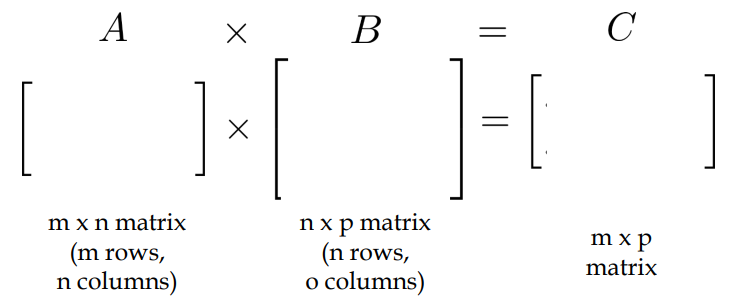
\includegraphics[width = 0.7\textwidth]{figs/matrix-matrix-mult.png}
\end{figure}

\subsection{Propiedades de la multiplicación de matrices}
\paragraph{No conmutatividad:} En general, la multiplicación de matrices no es conmutativa, es decir, $\vec{A} \times \vec{B} \neq \vec{B} \times \vec{A}$. Por ejemplo:
$$\begin{bmatrix}
1 & 1 \\ 0 & 0
\end{bmatrix} \times \begin{bmatrix}
0 & 0 \\ 2 & 0
\end{bmatrix} = \begin{bmatrix}
2 & 0 \\ 0 & 0
\end{bmatrix} $$

$$\begin{bmatrix}
0 & 0 \\ 2 & 0
\end{bmatrix} \times \begin{bmatrix}
1 & 1 \\ 0 & 0
\end{bmatrix} = \begin{bmatrix}
0 & 0 \\ 2 & 2
\end{bmatrix} $$

En el caso de multiplicar una matriz con una matriz de identidad, sí es conmutativa.

\paragraph{Matriz inversa} Si $\vec{A}$ es una matriz cuadrada $m \times m$, y tiene inversa, entonces
$$AA^{-1} = A^{-1}A = I$$

\paragraph{Transposición de matriz} Dada una matriz $A \in \mathbb{R}^{m \times n}$, su transpuesta $A^T$: es una matriz $n \times m$ donde $\forall i, j, \quad (A^T)_{ij} = A_{ji}$. Por ejemplo:
\begin{table}[h]
\centering
$A = \begin{bmatrix}
1 & 2 & 0 \\ 3 & 5 & 9
\end{bmatrix}$
\qquad \qquad \qquad
$A^T = \begin{bmatrix}
1 & 3 \\ 2 & 5 \\ 0 & 9
\end{bmatrix} $
\end{table}
% Luis -> meter el resto de operaciones y propiedades de https://stanford.edu/~shervine/teaching/cs-229/refresher-algebra-calculus (el finde quizá?).

\section{Introducción al Aprendizaje Automático o Machine Learning}
\subsection{Contexto histórico}
Hay muchas definiciones de aprendizaje automático. Según Wikipedia, machine learning es la construcción y estudio de sistemas que pueden aprender de datos. Arthur Samuel lo definía como un campo de estudio que confiere a los ordenadores la capacidad de aprender sin ser programados explícitamente. En el aprendizaje automático, no se diseña el algoritmo para que resuelva una tarea con unas reglas fijas, si no para que con una serie de datos pueda aprender a resolver la tarea. 

Arthur Samuel, en la década de 1950, escribió un programa para jugar a las damas que era capaz de aprender las mejores posiciones del tablero analizando miles de partidas. El sistema aprendió por sí mismo a jugar a las damas cada vez mejor. El 11 de mayo de 1997, el gran maestro de ajedrez Garry Kasparov renuncia tras 19 movimientos en una partida contra Deep Blue, un ordenador ajedrecista desarrollado por científicos de IBM. En 2016, Google (AlphaGo) derrotó al campeón mundial de Go. Este juego fue considerado durante décadas uno de los grandes retos de la IA. \footnote{Para el ajedrez, no se trata realmente de una inteligencia artificial, si no una máquina que calcula probabilidades. Cada movimiento proporciona una probabilidad de vencer al contrincante. Hay aperturas del ajedrez que facilitan un poco la victoria. Esto para el Go no existe. La máquina pudo encontrar una táctica para el Go nunca antes descrita, abriendo el debate de si se trata de creatividad.} En 2020, Google (AlphaFold) predice la estructura de las proteínas. Aquí se basa de \textbf{aprendizaje por refuerzo}. Se utilizó AlphaGo como base para generar otros modelos similares: AlphaChess, AlphaFold, etc. Las damas, el ajedrez, el go y las estructuras de las proteínas tienen en común ser problemas con unas reglas bien definidas. A partir de reglas sencillas, se generan estructuras complejas. Por ello, son campos donde se puede predecir o estimar muchas combinaciones y posibles variaciones. Estos algoritmos funcionan por prueba y error, por lo que no tiene sentido aplicarlo en otros campos donde los errores tienen consecuencias graves, como puede ser el diagnóstico de enfermedades o la conducción autónoma de coches. En general, todo el comportamiento humano es imposible de describir en reglas; cada paciente es muy complejo en sí mismo, siendo difícil generalizar en poblaciones grandes por procesos moleculares, comportamiento, epigenética, etc. 

La IA se ha democratizado mucho con los softwares open-source. Tecnológicamente no hay secretos a día de hoy, solo diferencias en los datos y el hardware. 

\subsection{De programación clásica al aprendizaje automático}
Los humanos adquieren con el tiempo experiencias que les hace aprender, causando respuestas concretas a distintas situaciones. Los ordenadores y las máquinas obtienen reglas predefinidas y datos, y con programación clásica llegan a su respuesta. No obstante, actualmente se utilizan datos y respuestas para, mediante aprendizaje automático, poder inferir las reglas. Esto invierte la forma de funcionar los ordenadores, y ha sido lo revolucionario del campo. Esas reglas inferidas se utilizarán para nuevos datos y poder ser cada vez más precisas. Así, el algoritmo encuentra las mejores reglas para resolver un problema. Estas reglas son ecuaciones matemáticas, pudiendo ser propensas a sesgos en base a los datos.

\subsection{De comportamiento humano a comportamiento computacional: el modelo estándar}
Una tarea humana se realiza a través de unos objetivos mediante abstracción. El proceso de aprendizaje está guiado por objetivos predefinidos (es decir, la simplificación de comportamientos complejos). En el caso de las máquinas,  el proceso de aprendizaje consta de etapas de optimización para llegar al objetivo. Al final se trata de una reducción y optimización de la abstracción humana. No obstante, no hay una visión directa entre el comportamiento de la máquina y el comportamiento humano. No se puede esperar que un algoritmo sea justo o generoso por naturaleza si no se especifica en sus objetivos. Por ello, es muy fácil que aparezcan sesgos en el aprendizaje automático. La toma de decisión es muy diferente entre un humano y una máquina.

\subsection{Cómo ve la IA: Un ejemplo con ataques adversarios}
Tenemos una imagen de un cerdo (figura \ref{fig:pig}), y no necesitamos el ruido para saber lo que es. Si le añadimos ruido a la imagen, aunque sea en una baja cantidad, la imagen no cambia para los humanos. No obstante, el sistema de reconocimiento de imágenes lo reconoce como una aerolínea. El ruido no es aleatorio, si no adversario. Esto quiere decir que la entrada al modelo ha sido modificada ligeramente de forma intencional, haciendo que el modelo genere una salida incorrecta. Se manipula para confundir a la máquina.

\begin{figure}[htbp]
\centering
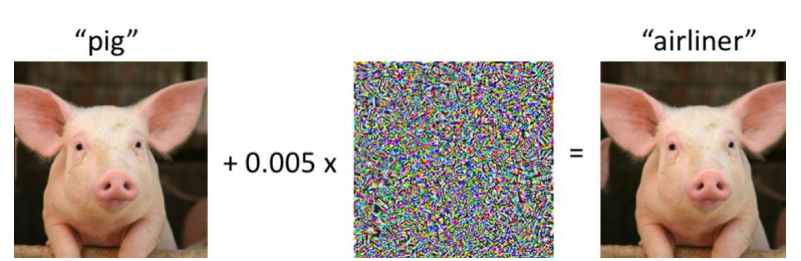
\includegraphics[width = 0.9\textwidth]{figs/pig-ai.png}
\caption{Reconocimiento de imágenes con ataque adversario.}
\label{fig:pig}
\end{figure}

\subsection{Cognición humana: sistema 1 vs sistema 2}
Los conceptos del libro Thinking, Fast and Slow de Daniel Kahneman se han aplicado en el campo del aprendizaje automático. Se habla de dos sistemas y categorías de tareas cognitivas. El \textbf{sistema 1} es intuitivo, rápido, inconsciente, no lingüístico y habitual. Se decía que el aprendizaje profundo estaba en ese sistema. El \textbf{sistema 2} es lento, lógico, secuencial, consciente, lingüístico, algorítmico, y es donde estaría el deep learning futuro. Esto sirvió para el aprendizaje automático de estructuras de datos: redes de cápsulas, aprendizaje automático neurosintáctico, razonamiento conceptual, bases de experiencia, reglas lógicas, etc. \textit{El sistema 1 sirve para reconocer formas, colores y posiciones, mientras que el sistema 2 ayuda en la predicción de interacciones.}

\subsection{Tarea de aprendizaje}
Se dice que un programa informático aprende de la experiencia E con respecto a alguna tarea T y alguna medida de rendimiento P, si su rendimiento en T, medido por P, mejora con la experiencia E. Si el rendimiento es perfecto desde el principio, no hay aprendizaje, ya que requiere una optimización o mejora del estado. Ejemplos son:
\begin{itemize}
\item T: Jugar a las damas \\ P: Porcentaje de partidas ganadas contra un contrincante arbitrario \\ E: Jugar partidas de práctica contra uno mismo
\item T: Reconocer palabras escritas a mano \\ P: Porcentaje de palabras clasificadas correctamente \\ E: Base de datos de imágenes de palabras manuscritas etiquetadas por humanos
\item T: Conducción en autopistas de cuatro carriles mediante sensores de visión \\ P: Distancia media recorrida antes de un error apreciado por el ser humano \\ E: Secuencia de imágenes y comandos de dirección grabados mientras se observa a un conductor humano.
\item T: clasificar los mensajes de correo electrónico como spam o legítimos. \\ P: Porcentaje de mensajes de correo electrónico clasificados correctamente. \\ E: Base de datos de correos electrónicos, algunos con etiquetas dadas por humanos.
\end{itemize}

\subsection{Aprendizaje automático en contexto}
En el núcleo de la IA, el aprendizaje automático es simplemente una forma de conseguir IA. En lugar de codificar rutinas de software con instrucciones específicas para realizar una tarea concreta, el ML es una forma de «entrenar» un algoritmo para que aprenda a hacerlo. El «entrenamiento» consiste en introducir grandes cantidades de datos en el algoritmo y permitir que éste se ajuste y mejore.

\begin{figure}[htbp]
\centering
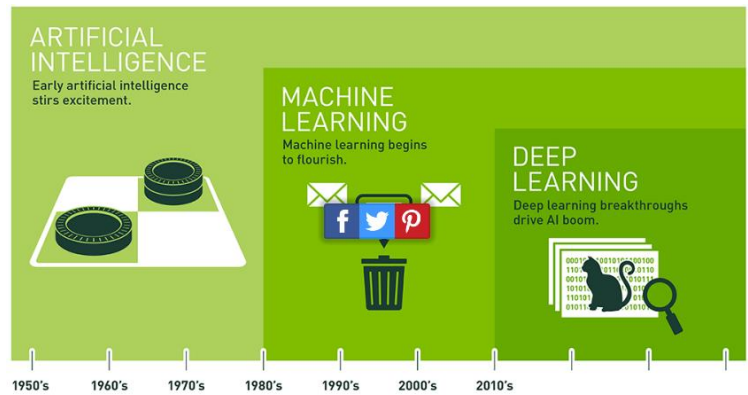
\includegraphics[width = 0.8\textwidth]{figs/ai-timeline.png}
\caption{Mapa temporal del desarrollo de las inteligencias artificiales. Ya está algo desfasado, faltaría añadir después del Deep Learning los Modelos Generativos.}
\end{figure}

No se trata de comparar el aprendizaje humano vs aprendizaje automático, si no combinar ambos para sacar lo mejor de los dos mundos. Habrá tareas que se irán automatizando.

\subsection{Diseño de sistema de aprendizaje}
Muchos métodos de aprendizaje implican formación. La formación es la adquisición de conocimientos, destrezas y competencias como resultado de la enseñanza de aptitudes o conocimientos prácticos relacionados con una competencia útil. La formación requiere escenarios o ejemplos (datos). Existen varios tipos de sistemas de aprendizaje:
\begin{itemize}
\item \textbf{Aprendizaje no supervisado:} No se proporcionan respuestas o retroalimentación explícita. El sistema debe encontrar patrones o estructuras en los datos por sí mismo.
\item \textbf{Aprendizaje supervisado:} Se utiliza un conjunto de datos etiquetados, es decir, se proporcionan ejemplos con las respuestas correctas. El sistema aprende a mapear las entradas (x) a las salidas (y) basándose en estos ejemplos.
\item \textbf{Aprendizaje de refuerzo:} La retroalimentación es indirecta y se recibe después de varias acciones o decisiones. El sistema aprende a través de la interacción con un entorno, recibiendo recompensas o penalizaciones.
\end{itemize}

\subsubsection{Supervisado vs no supervisado}
Supongamos una función desconocida $y_{\Theta}(\vec{x}) = h_{\Theta}(\vec{x})$, donde x es un ejemplo de entrada y y la salida deseada. En el \textbf{aprendizaje supervisado}, se proporciona un conjunto de pares de entrenamiento (x,y), donde x es la entrada y y es la salida deseada. El objetivo es aprender una función $h_{\Theta}(\vec{x})$ que mapee las entradas a las salidas. En el \textbf{aprendizaje no supervisado}, solo se proporcionan las entradas x, y el sistema debe encontrar patrones o estructuras en los datos sin conocer las salidas. $\Theta$ hace referencia a los parámetros que tiene el modelo y que hay que entrenar. Por tanto, cuantos menos parámetros haya, más rápido va a ser el modelo.

\subsubsection{Fases de un algoritmo de aprendizaje}
Las fases de un algoritmo de aprendizaje son:
\begin{enumerate}
\item \textbf{Hipótesis y datos}: Los datos son representados como vectores\footnote{Aunque no haya una notación general, vamos a utilizar la negrita no itálica para denominar que la variable es un vector. }  $\vec{x}_n = (x_{n1} ... x_{nD})^T$, donde D es la dimensión del vector. En el aprendizaje supervisado, también se tienen etiquetas $y_n$ que representan la salida deseada. Los datos pueden ser de diferentes tipos: numéricos, categóricos, texto, series temporales, etc. La información puede estar estructurada (datos genéticos, metereológicos, etc) o no estructurada (imágenes, audio, texto).

\item \textbf{Selección del modelo}

Se elige un modelo $h_{\Theta}(\vec{x})$ que intenta aproximar la relación entre las entradas y las salidas. Por ejemplo, si se elige un modelo lineal, $h_{\Theta}(\vec{x}) = a\vec{x} + b$, donde a y b son parámetros que se deben optimizar (correspondientes a $\Theta_1$ y a $\Theta_2$). 

\begin{figure}[h]
\centering
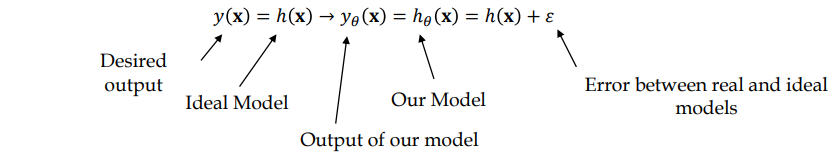
\includegraphics[width = \textwidth]{figs/model-htheta.png}
\end{figure}

La función de coste $E(y_{\Theta} - y )^2$ mide el error entre la predicción del modelo y la salida real. Este error se divide en un coste reducible que se puede minimizar optimizando los parámetros del modelo, y un coste irreducible que no puede reducirse con los parámetros actuales, requiriendo un cambio en el modelo o la hipótesis. La función del coste se resume en:
$$E(y_{\Theta} - y)^2 = [h_{\Theta}(\vec{x}) - h(\vec{x})]^2 + \epsilon$$

siendo $ [h_{\Theta}(\vec{x}) - h(\vec{x})]^2$ el coste reducible y $\epsilon$ el irreducible. 

\item \textbf{Entrenamiento o aprendizaje}: En esta fase, el modelo se ajusta a los datos de entrenamiento optimizando los parámetros $\Theta$ para minimizar la función de coste.

Por ejemplo, si tenemos un set de datos logarítmico, habría que cambiar de la hipótesis de modelo lineal $h_{\Theta}(x) = ax + b$ que solo valdría para una recta, por un modelo polinómico $h_{\Theta}(x) = ax^3 + bx^2 + cx + d$ para poder disminuir el error $\epsilon$. El problema es que es muy costoso matemáticamente cuando aumenta el tamaño de los datos, y puede llevar a un sobreajuste del modelo a los datos de entrenamiento. De una información discreta (un set de valores) se busca obtener una solución continua (la función). Todo esto no solo permite obtener una aproximación de los datos intermedios del set de valores dado, si no también una predicción de los datos futuros.

Los errores se suelen representar al cuadrado para que no se compensen los errores negativos con los positivos. 

\item \textbf{Testeo o inferencia}: Una vez entrenado, el modelo $h_{\Theta}$ se evalúa con datos nuevos (no vistos durante el entrenamiento) para ver cómo generaliza a situaciones no vistas. Así, se predice un nuevo $y(\vec{x})$ a un nuevo $\vec{x}$. Esto normalmente se hace separando un set de datos en un set de entrenamiento y un set de evaluación de forma aleatoria. 

Una vez en este punto, si el error es muy elevado, se vuelve a la selección del modelo y se establece una nueva hipótesis. Esto es un proceso iterativo en el que se evalúa el rendimiento del sistema hasta que se observe un modelo con un buen ajuste tanto a los valores de entrenamiento como a los valores de test.
\end{enumerate}

\subsection{Tipos de problemas o tareas}
\subsubsection{Aprendizaje supervisado}
\paragraph{Regresión} El objetivo de la regresión es predecir el valor de una variable continua. La salida es un valor numérico, y se busca modelar una función continua que relacione las variables de entrada con la salida. Este proceso implica métodos estadísticos para estimar las relaciones entre las variables. Por ejemplo, predecir el precio de una casa en función de su tamaño, ubicación y otras características.

\paragraph{Clasificación} En la clasificación, el objetivo es asignar una etiqueta categórica a cada instancia de datos. La salida es una etiqueta discreta, como "maligno" o "benigno". El límite de decisión es una hipersuperficie que divide el espacio de características en regiones, cada una asociada a una clase. Por ejemplo, en la clasificación de un tumor, se utilizan características como el tamaño y la tasa de crecimiento para determinar si el tumor es maligno o benigno. Aquí, las características (tamaño y tasa de crecimiento) definen el espacio de entrada, y la etiqueta (maligno/benigno) es la salida binaria.

\subsubsection{Aprendizaje no supervisado}
\paragraph{Clustering} El clustering es una técnica de aprendizaje no supervisado que busca agrupar un conjunto de objetos (o datos) de manera que aquellos que pertenecen al mismo grupo (clúster) sean más similares entre sí que con los objetos de otros grupos. La similitud se mide utilizando métricas de distancia (como la distancia euclidiana) o similitud, dependiendo del tipo de datos y del algoritmo utilizado. Un ejemplo común es la agrupación de clientes en segmentos basados en su comportamiento de compra, donde cada clúster representa un grupo de clientes con características similares.

%04/02 - Aythami
\section{Reducción de dimensionalidad}
La reducción de dimensionalidad es una técnica fundamental en el aprendizaje automático que permite representar datos multidimensionales en un espacio de menor dimensión, preservando la mayor cantidad posible de información relevante. Esto es especialmente útil para visualización, mejora del rendimiento y manejo de la maldición de la dimensionalidad. 
\begin{itemize}
\item \textbf{Visualización}: Permite visualizar datos en 2D o 3D, incluso cuando los datos originales tienen muchas más dimensiones.
\item \textbf{Mejora del rendimiento}: Reduce el tiempo de entrenamiento y el uso de memoria al trabajar con menos dimensiones. Además, elimina ruido y redundancia en los datos.
\item \textbf{Maldición de la dimensionalidad}: Cuando el número de dimensiones es muy alto en comparación con el número de muestras, los modelos pueden volverse ineficientes o sobreajustarse.
Ejemplo: No tiene sentido ajustar un modelo con 2.000 parámetros si solo se dispone de 10 datos. Los parámetros representan grados de libertad, y en este caso, el modelo no generalizaría bien. La reducción de dimensionalidad ayuda a eliminar información redundante y mejorar el rendimiento.
\end{itemize}

No obstante, no siempre es necesario o beneficioso reducir la dimensionalidad. Por ejemplo, si las dimensiones originales ya son interpretables y no hay redundancia, o si la pérdida de información al reducir dimensiones afecta negativamente al modelo.

El objetivo es reducir el número de variables (dimensiones) en un conjunto de datos, manteniendo la estructura y la información más importante. La herramienta más común es \textbf{PCA (Principal Component Analysis)}, un algoritmo basado en álgebra lineal que transforma los datos originales en un nuevo sistema de coordenadas, donde las dimensiones (componentes principales) capturan la mayor varianza posible.

\subsection{Proyección de datos en dimensiones inferiores}
La idea central de la reducción de dimensionalidad es proyectar datos de un espacio de alta dimensión a uno de menor dimensión, preservando la estructura subyacente.

\paragraph{2D a 1D}
Supongamos que tenemos datos en un espacio bidimensional ($\mathbb{R}^2$). Queremos proyectarlos en una recta unidimensional ($\mathbb{R}$). La recta es una combinación lineal de las dos dimensiones originales (desde la recta, solo nos podemos mover en una dirección, hacia delante o hacia detrás), y la proyección de los datos a esa recta no conlleva pérdida de información si la recta captura la dirección de máxima varianza. Matemáticamente:
$$\vec{x}^{(1)} \in \mathbb{R}^2 \rightarrow z^{(1)} \in \mathbb{R}$$
$$\vec{x}^{(2)} \in \mathbb{R}^2 \rightarrow z^{(2)} \in \mathbb{R}$$
$$\vec{x}^{(N)} \in \mathbb{R}^2 \rightarrow z^{(N)} \in \mathbb{R}$$
El superíndice sirve para anotar el dato, y el subíndice para la dimensión.

\begin{figure}[h]
\centering
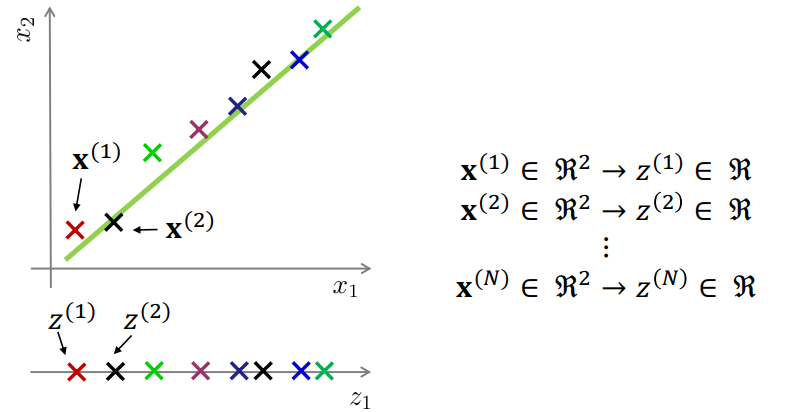
\includegraphics[width = 0.6\textwidth]{figs/reduccion-dimension-2d.png}
\end{figure}

\paragraph{Extensión a más dimensiones}
Esta idea se puede generalizar a espacios de mayor dimensión. Por ejemplo, al pasar de 3D ($\mathbb{R}^3$) a 2D ($\mathbb{R}^2$), se proyectan los datos en un plano bidimensional:
$$\vec{x}^{(i)} \in \mathbb{R}^3 \rightarrow z^{(i)} \in \mathbb{R}^2$$

\subsection{PCA: Análisis de Componentes Principales}
El Análisis de Componentes Principales (PCA) es una técnica de reducción de dimensionalidad que transforma datos de alta dimensión en un espacio de menor dimensión, preservando la mayor cantidad posible de información (varianza). Es especialmente útil cuando se trabaja con datos multidimensionales, como en el caso de una \textbf{tabla de expresión génica}, donde las filas representan pacientes y las columnas corresponden a genes individuales.

\paragraph{Ejemplo: Tabla de expresión génica}
Cada paciente puede describirse como un punto en un espacio de 2000 dimensiones: $\vec{x}^{(i)} \in \mathbb{B}^{2000}$,  donde cada componente del vector representa la expresión de un gen.
PCA permite reducir estas 2000 dimensiones a un espacio de menor dimensión, por ejemplo, a dos dimensiones: $\vec{z}^{(i)} \in \mathbb{R}^2$.

Nota: Al proyectar los datos, los valores transformados pierden su significado biológico directo (ya no representan expresiones génicas específicas). Sin embargo, la proximidad entre puntos en el espacio bidimensional puede interpretarse como una medida de similitud genética entre pacientes.

\begin{figure}[h]
\centering
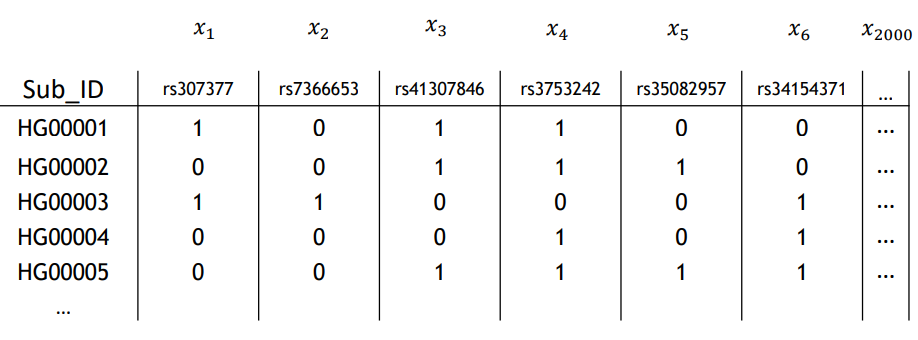
\includegraphics[width = 0.7\textwidth]{figs/gene-table1.png}
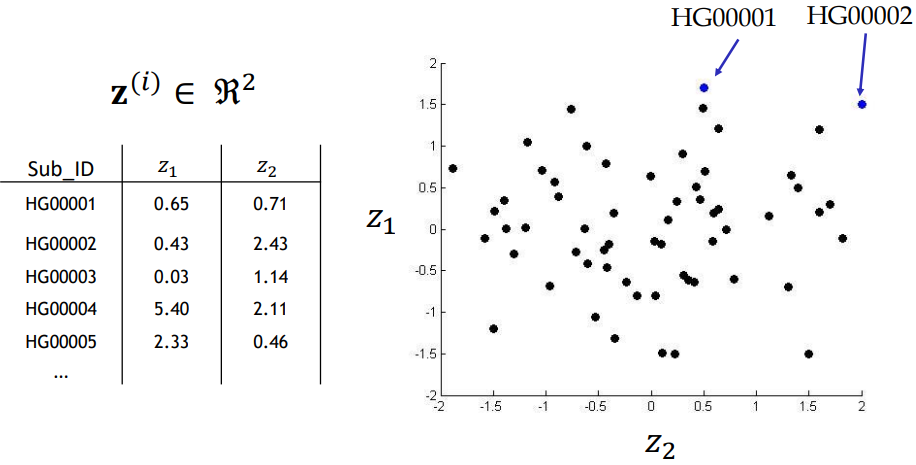
\includegraphics[width = 0.7\textwidth]{figs/gene-table2.png}
\end{figure}

PCA busca minimizar el error de proyección de los datos sobre un subespacio de menor dimensión. Para reducir un espacio de $n$ dimensiones a $k$ dimensiones, PCA determina $k$ vectores ortogonales $\vec{u}^{(k)}$ que definen el subespacio óptimo para proyectar los datos:

$$\vec{x} \in \mathbb{R}^n \rightarrow \vec{z} \in \mathbb{R}^k$$

\begin{figure}[h]
\centering
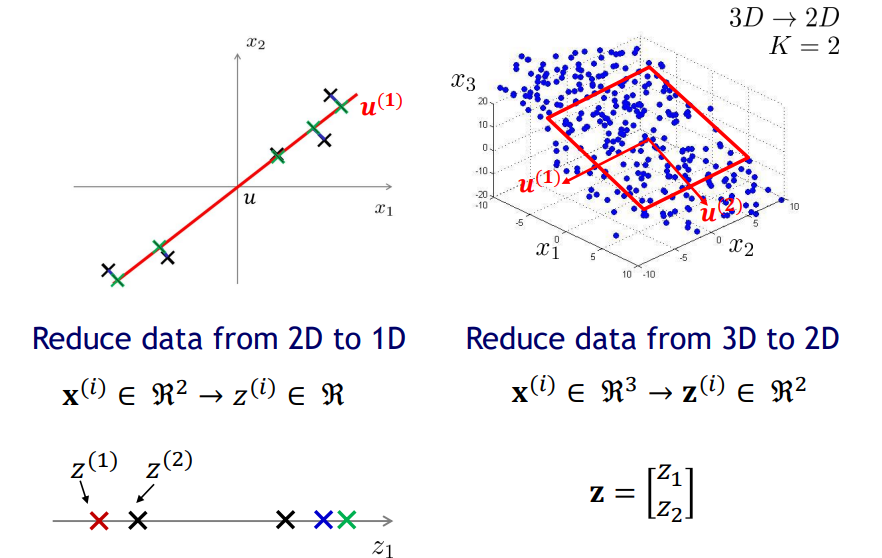
\includegraphics[width = 0.8\textwidth]{figs/pca-dimensiones.png}
\end{figure}

%10/02 - Aythami
\subsubsection{Algoritmo de PCA}
La recta z es una combinación lineal de las variables x1 y x2 (sumas y multiplicaciones por escalares). 
$$\vec{z}_1 = a\vec{x}_1 + b\vec{x}_2$$
El problema es el rango de las dos variables; quizás una está en el rango de las unidades, y la otra en los miles. Para llevar los datos a un rango común, se puede restar la media a la distribución, de forma que las dos distribuciones estén centradas en 0. Ahora, el rango de varianza sigue siendo muy diferente, por lo que se divide por la desviación estándar. A esto se conoce como pre-procesado o normalización basada en media/varianza. 
$$x_j^{(i)} = \frac{x_j^{(i)} - \mu_j}{\delta_j}$$
Esto no es un paso necesario de PCA si las variables no son tan distantes y son perfectamente combinables. 

Siendo $\vec{x}$ la matriz, M es el número de datos o de filas, y N el número de características. Se calcula la matriz de covarianza de $\vec{x}$ que se obtiene mediante una fórmula matemática o mediante operaciones con matrices. Se obtiene la correlación que existe entre las distintas variables de la matriz en las distintas celdas y entre la propia variable en la diagonal principal. La matriz de covarianza no depende de M, indicando que hay que tener en cuenta la robutez estadística.
$$\vec{x} \in \mathbb{R}^{M \times N} \rightarrow \Sigma \in \mathbb{R}^{n \times n}$$

A la matriz de covarianza hay que computar los autovalores. Los autovectores están relacionados con las direcciones en los que se mueven los datos dentro de la matriz. La matriz tiene datos, los cuales se mueven en unas direcciones, es decir, la distribución en las variables. Además, cada variable es ortogonal (perpendicular). Los autovalores son la cantidad de información que se distribuye en esa dirección. No va a ser 100\%. Los autovalores están relacionados con la varianza que hay en la dimensión. Autovector U = direcciones en las que se distribuyen los datos. Autovalor lambda = cantidad de información que se distribuye en la dirección. 
$$\lambda = \begin{bmatrix}
\lambda_1 \\ ... \\ \lambda_n
\end{bmatrix} \in \mathbb{R}^{n \times 1}$$

$$\vec{U} = \begin{pmatrix}
\vec{u}^{(i)} & ... & \vec{u}^{(n)}
\end{pmatrix} \in \mathbb{R}^{n \times n} $$

En PCA se busca el punto de vista, transformando los datos, para minimizar el error de proyección y resaltar patrones. 

Autovalores hay tantos como dimensiones que tiene el problema (número de variables), mientras que los autovectores tienen una dimensión n x n. Existe el mismo número de autovectores como autovalores, pero los autovectores están compuestos por dos números. 

Los autovalores se ordenan de mayor a menor, generando un vector lambda prima ordenado. Se ordena la matriz de transición U en base al orden de lambda prima. 

Para reducir dimensionalidad, se descartan autovectores. En caso de tener dos, desechamos el segundo y nos quedamos solo con el primero. 
$$U' = \begin{bmatrix}
-1 & 2 \\ 
3 & 0
\end{bmatrix}$$
U es de dimensión n x n, por lo que va a ser siempre cuadrado, pero no podemos conocer el valor de M. Para proyectar a una dimensión, nos debemos quedar con
$$\breve{U} = \begin{bmatrix}
-1 \\ 3
\end{bmatrix}$$

$$z = \breve{U}^T x$$
$$\breve{U} \in \mathbb{R}^{n \times k}$$
$$x \in \mathbb{R}^{n \times 1}$$
Al transponer, se queda en dimensiones $k \times n$, coincidiendo con la primera dimensión de la otra variable. El resultado de la multiplicación matricial es un vector de dimensiones $k \times 1$. 
Siguiendo con el ejemplo:
$$z = \begin{bmatrix}
-1 & 3
\end{bmatrix} \begin{bmatrix}
x_1 \\ x_2
\end{bmatrix}$$

En caso de no reducir dimensiones:
$$z = \begin{bmatrix}
-1 & 3 \\ 2 & 0
\end{bmatrix} \begin{bmatrix}
x_1 \\ x_2
\end{bmatrix} = \begin{bmatrix}
-1 x_1 + 3 x_2 \\
2 x_1 + 0 x_2
\end{bmatrix} \sim \begin{bmatrix}
z_1 \\ z_2
\end{bmatrix}$$

\begin{figure}[h]
\centering
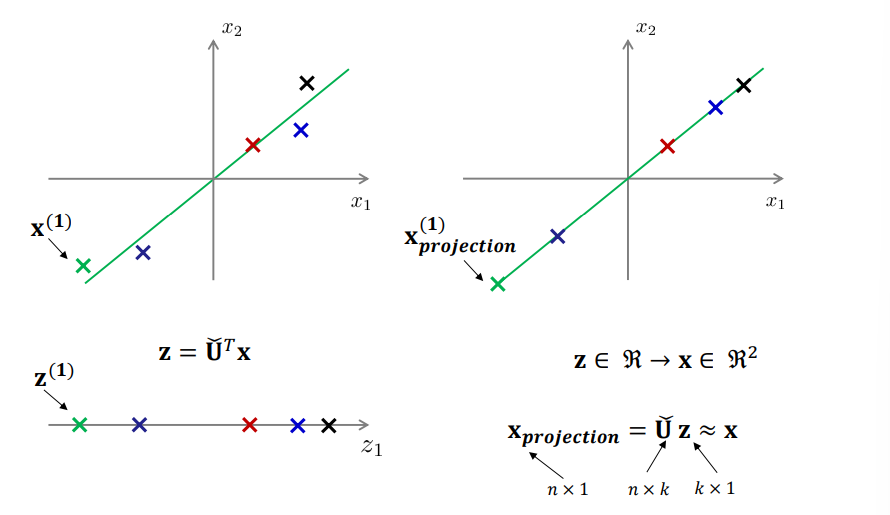
\includegraphics[width = 0.8\textwidth]{figs/resumen-PCA.png}
\end{figure}

\subsubsection{Escoger el número de componentes principales}
Se suele escoger la varianza explicada. Los autovalores dan un valor relacionado con la cantidad de información en cada autovector. Al pasar de dos dimensiones a una, la varianza explicada con la variable 1 es $\lambda_1 / \lambda_1 + \lambda_2$.